% Propósito: relacionar un ángulo del círculo unitario con coseno y seno.
% Origen: x=cos(theta), y=sin(theta) para un radio unitario.
% Descripción accesible: en un círculo de radio uno, un radio forma un ángulo
% theta con el eje horizontal. La proyección horizontal del punto extremo mide
% cos(theta) y la proyección vertical mide sin(theta).
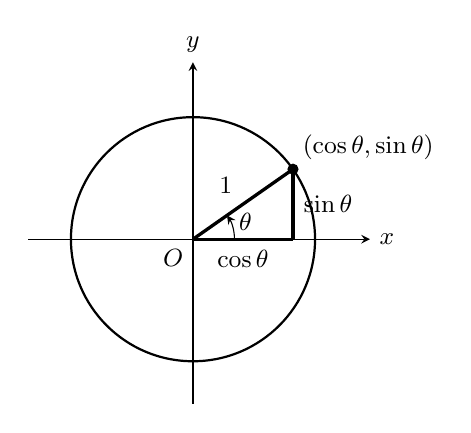
\begin{tikzpicture}[font=\small,>=stealth,scale=1.55]
    \draw[->] (-1.35,0) -- (1.45,0) node[right]{\(x\)};
    \draw[->] (0,-1.35) -- (0,1.45) node[above]{\(y\)};
    \draw[thick] (0,0) circle (1);

    \coordinate (P) at (35:1);
    \coordinate (Px) at ({cos(35)},0);

    \draw[very thick] (0,0) -- node[above left]{\(1\)} (P);
    \draw[dashed] (P) -- (Px);
    \draw[very thick] (0,0) -- node[below]{\(\cos\theta\)} (Px);
    \draw[very thick] (Px) -- node[right]{\(\sin\theta\)} (P);
    \fill (P) circle (1.3pt);

    \draw[->] (0.34,0) arc[start angle=0,end angle=35,radius=0.34];
    \node at (0.43,0.14) {\(\theta\)};

    \node[below left] at (0,0) {\(O\)};
    \node[above right] at (P) {\((\cos\theta,\sin\theta)\)};
\end{tikzpicture}
